\section{Motivation}

%As a motivation example, consider...

%Here we give an example to motivate our work. E.g. assuming we have a zero-cost profiling based work metric,
%how can we use it to perform iterative compilation across runs? Then we talk about while it is impossible to
%build a zero-overhead metric, we can develop one with low overhead.

This section provides a comparison between the offline and online approaches for
{\itercomp}.
The goal is to motivate the need for an online {\itercomp}, highlighting
weaknesses of using offline {\itercomp}.

In the offline approach, a fixed set of inputs is selected for which the best
optimization sequence is selected during the development time (pre-shipping) of
a program.
Although this fixed set of inputs is expected to be representative of the user's
workload,
in most cases, it might be infeasible to identify and collect representative
workloads for every group of users.
Furthermore, a user can dynamically change its workload pattern, rendering
a fixed optimization sequence innapropriate for his performance requirements.

In the online approach, the program is shipped with an initial optimization
sequence and different optimization sequences are evaluated as the end-user
executes the program.
This approach frees developers from the need to collect representative
workloads for every group of users so that the program can be optimized
accordingly.
More importantly, even in scenarios where the user's workload can dynamically
change its pattern, the online {\itercomp} would still be able to optimize the
program accordingly.

Figure~\ref{fig:motivation} compares the offline {\itercomp} with a potential
implementation of the online {\itercomp}.
For this experiment, we have executed the program twice for each input
in order to compute the speedup of the optimization sequence being evaluated.
This figure shows the performance gains of the best optimization 
sequence found by each approach, compared with the standard
compiler's optimization (i.e.,\texttt{-O3}), executed with 1,000 inputs.
Both approaches used the same set of optimization sequences, but because
the online {\itercomp} compares optimization sequences across inputs,
it is better informed throughout the search.

\begin{figure}[ht]
    \centering
    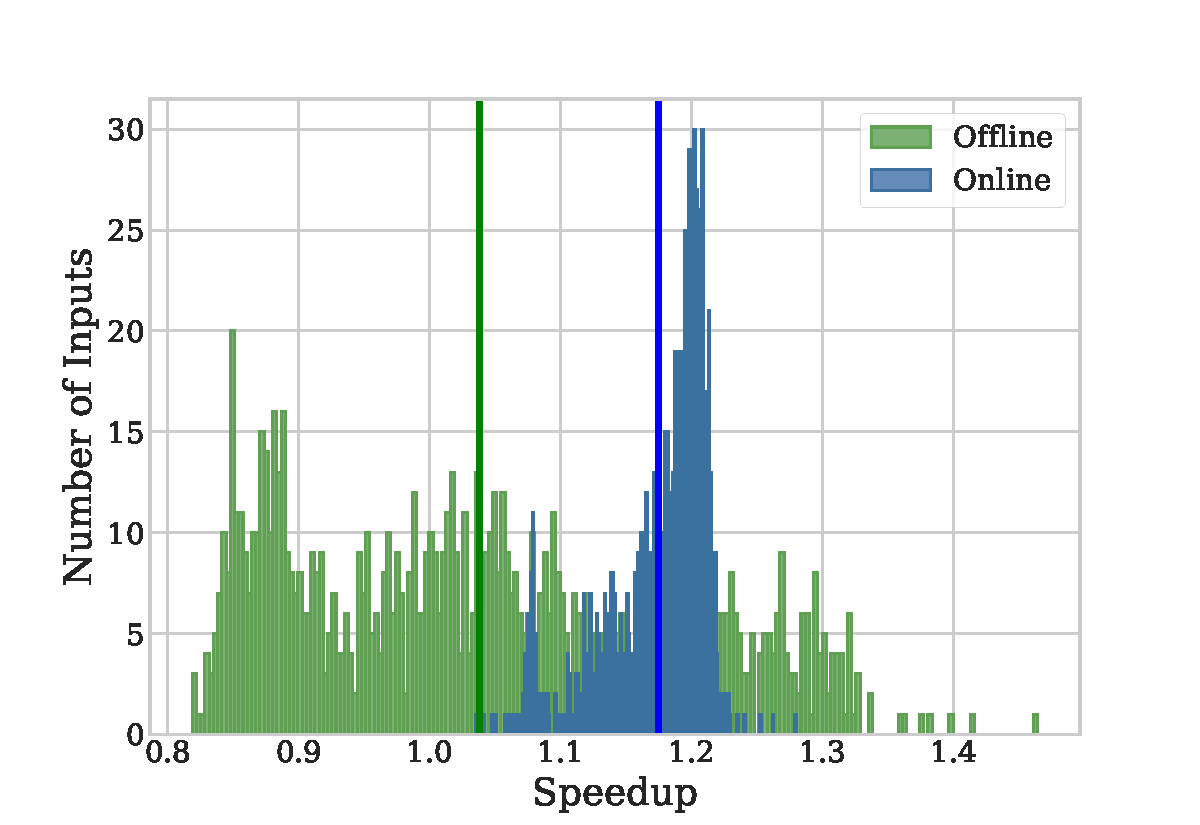
\includegraphics[width=0.5\textwidth]{figs/motivation.pdf}
    \caption{Comparison between the offline and online {\itercomp}.
             The vertical lines represent the average speedups over
             all the 1,000 inputs.
             }
    \label{fig:motivation}
\end{figure}


However, because of the restriction of having a single execution per input,
it is not possible to measure speedup in a real-world online scenario.
Moreover, measuring just execution time, for example, is also not viable since
different inputs often mean different amounts of work,
rendering it meaningless to compare optimizations only by execution time.

In the remaining of this paper we develop a work efficiency metric, suitable
for guiding online {\itercomp}, which can be profiled with a single execution
of the program with the optimization sequence being evaluated.

